\documentclass[11pt,a4paper]{report}
\usepackage[textwidth=37em,vmargin=30mm]{geometry}
\usepackage{calc,xunicode,amsmath,amssymb,paralist,enumitem,tabu,booktabs,datetime2,xeCJK,xeCJKfntef,listings}
\usepackage{tocloft,fancyhdr,tcolorbox,xcolor,graphicx,eso-pic,xltxtra,xelatexemoji}

\newcommand{\envyear}[0]{2025}
\newcommand{\envdatestr}[0]{2025-04-18}
\newcommand{\envfinaldir}[0]{webdb/2025/20250418/final}

\usepackage[hidelinks]{hyperref}
\hypersetup{
    colorlinks=false,
    pdfpagemode=FullScreen,
    pdftitle={Web Digest - \envdatestr}
}

\setlength{\cftbeforechapskip}{10pt}
\renewcommand{\cftchapfont}{\rmfamily\bfseries\large\raggedright}
\setlength{\cftbeforesecskip}{2pt}
\renewcommand{\cftsecfont}{\sffamily\small\raggedright}

\setdefaultleftmargin{2em}{2em}{1em}{1em}{1em}{1em}

\usepackage{xeCJK,xeCJKfntef}
\xeCJKsetup{PunctStyle=plain,RubberPunctSkip=false,CJKglue=\strut\hskip 0pt plus 0.1em minus 0.05em,CJKecglue=\strut\hskip 0.22em plus 0.2em}
\XeTeXlinebreaklocale "zh"
\XeTeXlinebreakskip = 0pt


\setmainfont{Brygada 1918}
\setromanfont{Brygada 1918}
\setsansfont{IBM Plex Sans}
\setmonofont{JetBrains Mono NL}
\setCJKmainfont{Noto Serif CJK SC}
\setCJKromanfont{Noto Serif CJK SC}
\setCJKsansfont{Noto Sans CJK SC}
\setCJKmonofont{Noto Sans CJK SC}

\setlength{\parindent}{0pt}
\setlength{\parskip}{8pt}
\linespread{1.15}

\lstset{
	basicstyle=\ttfamily\footnotesize,
	numbersep=5pt,
	backgroundcolor=\color{black!5},
	showspaces=false,
	showstringspaces=false,
	showtabs=false,
	tabsize=2,
	captionpos=b,
	breaklines=true,
	breakatwhitespace=true,
	breakautoindent=true,
	linewidth=\textwidth
}






\newcommand{\coverpic}[2]{
    % argv: itemurl, authorname
    Cover photo by #2~~(\href{#1}{#1})
}
\newcommand{\makeheader}[0]{
    \begin{titlepage}
        % \newgeometry{hmargin=15mm,tmargin=21mm,bmargin=12mm}
        \begin{center}
            
            \rmfamily\scshape
            \fontspec{BaskervilleF}
            \fontspec{Old Standard}
            \fontsize{59pt}{70pt}\selectfont
            WEB\hfill DIGEST
            
            \vfill
            % \vskip 30pt
            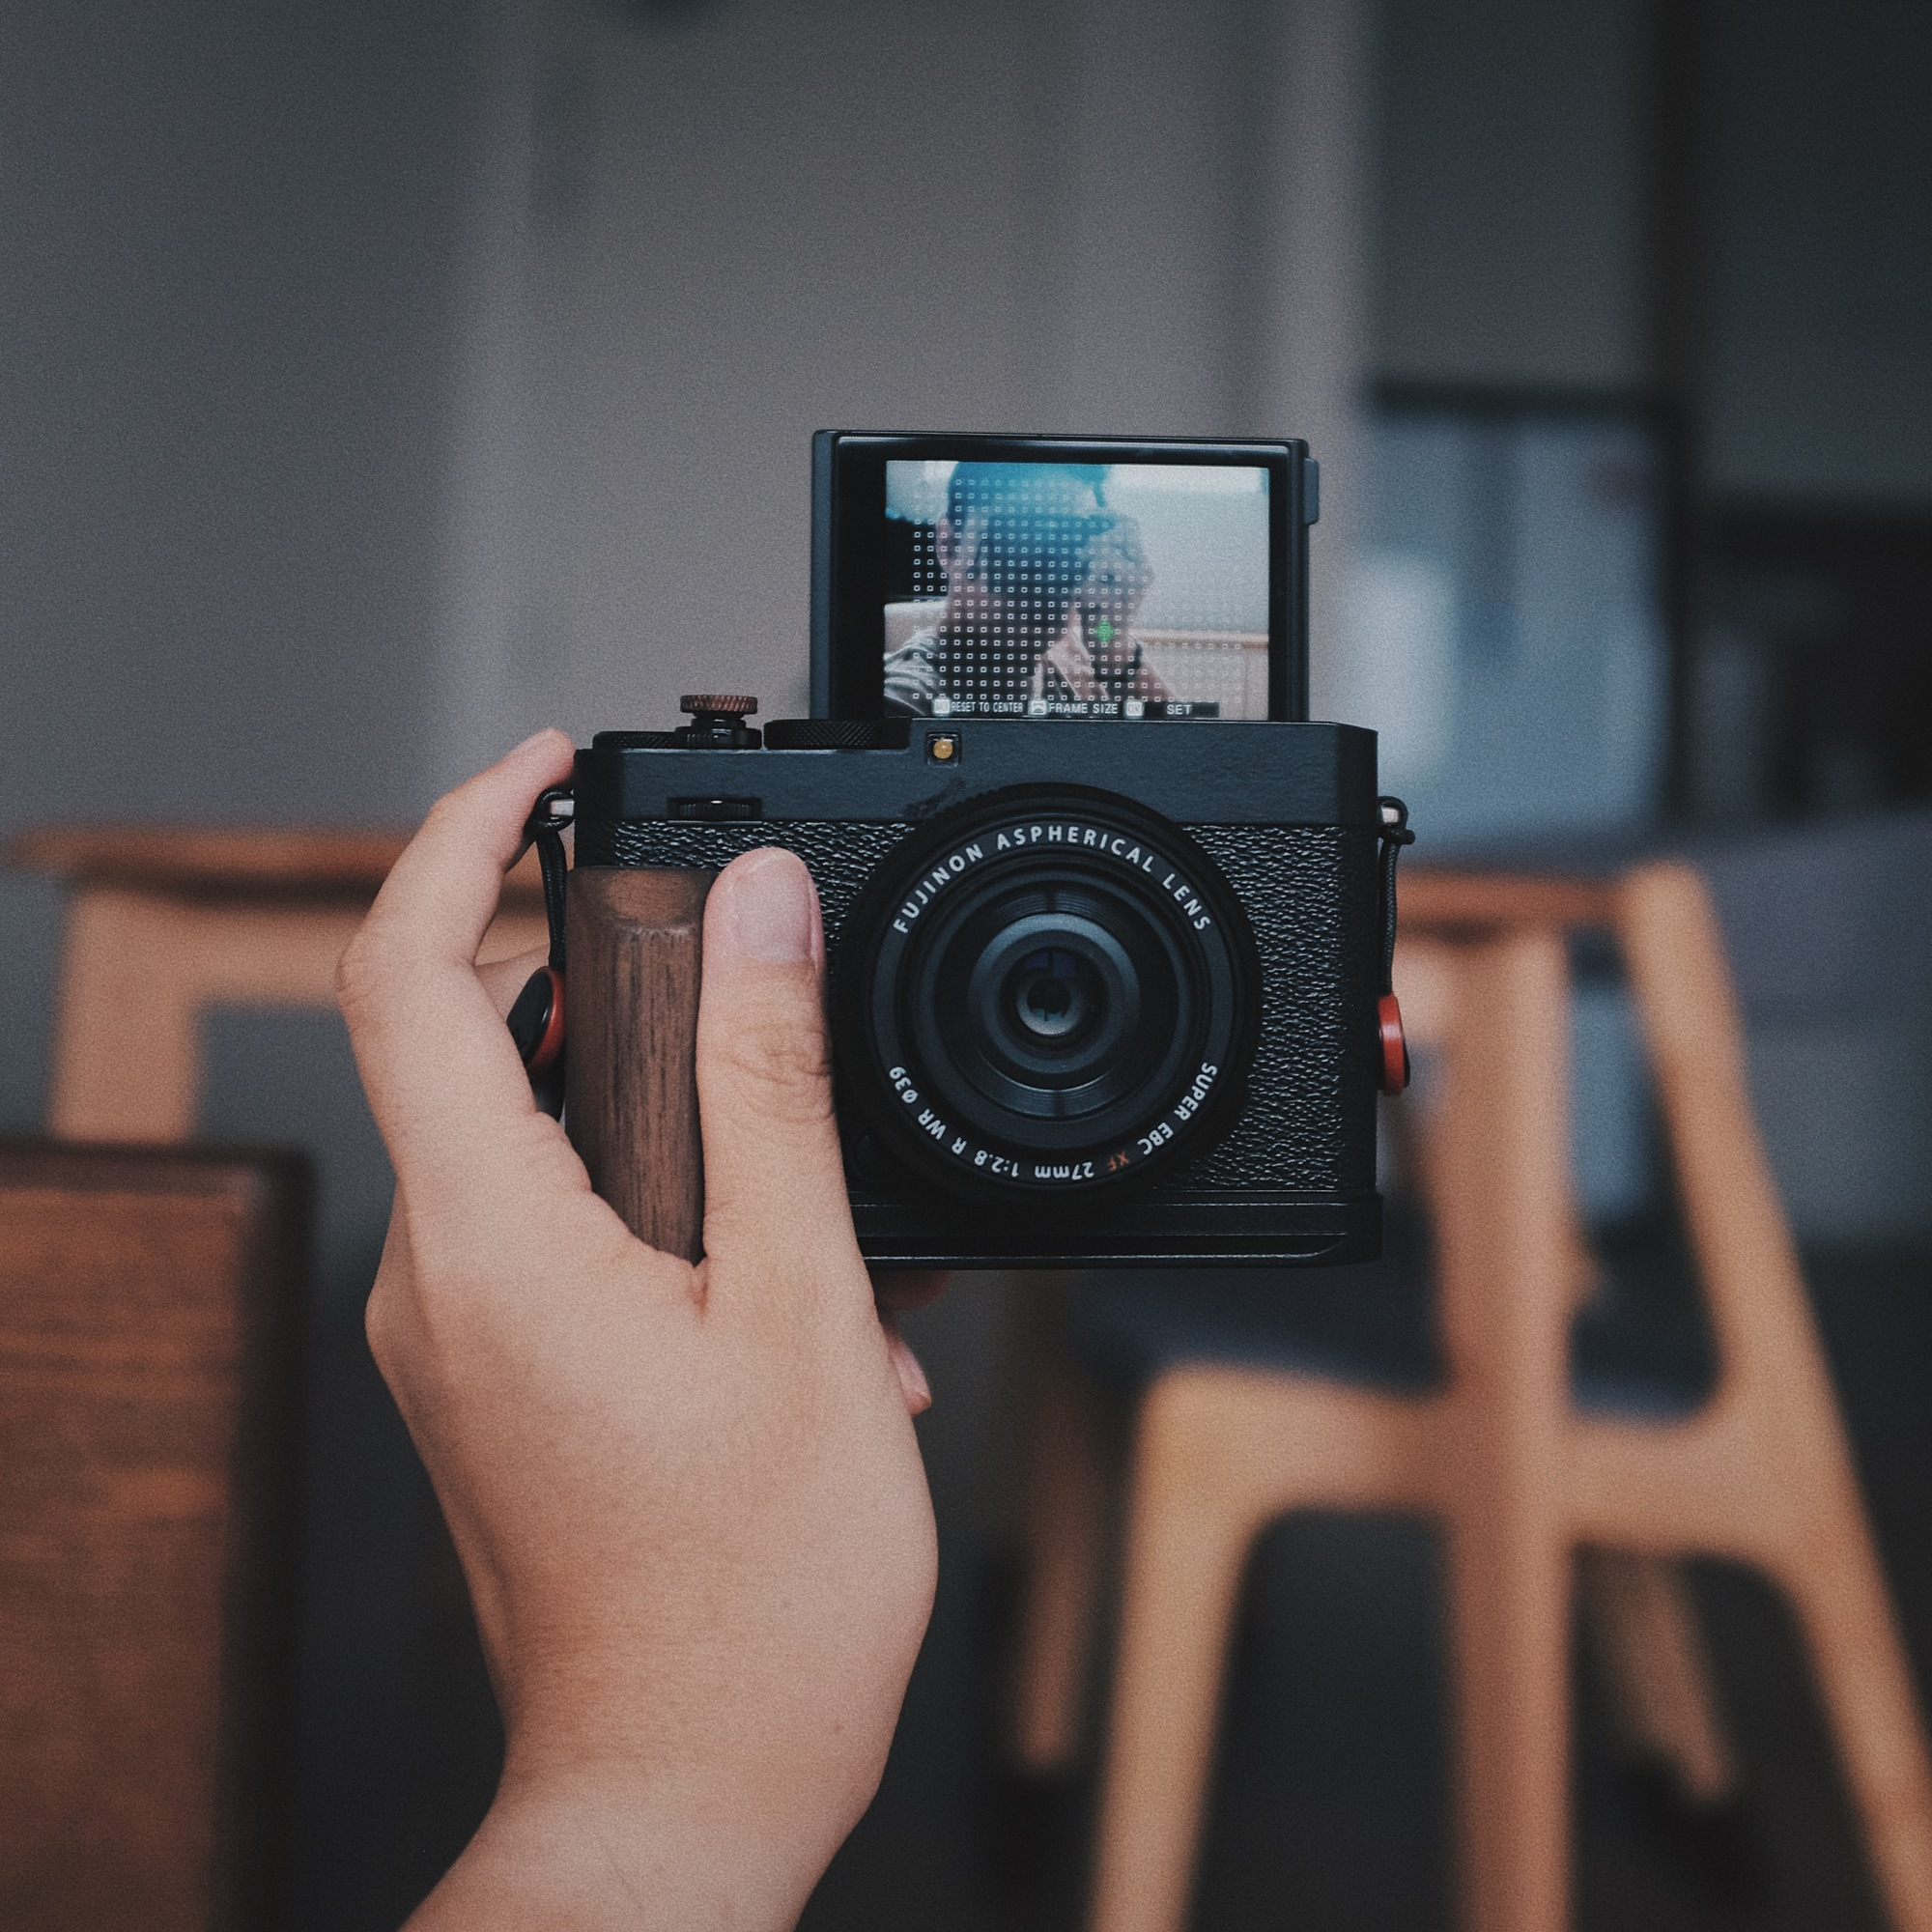
\includegraphics[width=\linewidth]{\envfinaldir/coverpic-prod.jpg}\par
            % \vskip 30pt
            \vfill

            \normalsize\rmfamily\scshape
            \copyright{} The Web Digest Project \hfill\large \envdatestr
        \end{center}
    \end{titlepage}
    % \restoregeometry
}
\newcommand{\simplehref}[1]{%
    \textcolor{blue!80!green}{\href{#1}{#1}}%
}
\renewcommand{\contentsname}{\center\Huge\sffamily\bfseries Contents\par\vskip 20pt}
\newcounter{ipartcounter}
\setcounter{ipartcounter}{0}
\newcommand{\ipart}[1]{
    % \vskip 20pt
    \clearpage
    \stepcounter{ipartcounter}
    \phantomsection
    \addcontentsline{toc}{chapter}{#1}
    % \begin{center}
    %     \Huge
    %     \sffamily\bfseries
    %     #1
    % \end{center}
    % \vskip 20pt plus 7pt
}
\newcounter{ichaptercounter}
\setcounter{ichaptercounter}{0}
\newcommand{\ichapter}[1]{
    % \vskip 20pt
    \clearpage
    \stepcounter{ichaptercounter}
    \phantomsection
    \addcontentsline{toc}{section}{\numberline{\arabic{ichaptercounter}}#1}
    \begin{center}
        \Huge
        \sffamily\bfseries
        #1
    \end{center}
    \vskip 20pt plus 7pt
}
\newcommand{\entrytitlefont}[1]{\subsection*{\raggedright\Large\sffamily\bfseries#1}}
\newcommand{\entryitemGeneric}[2]{
    % argv: title, url
    \parbox{\linewidth}{
        \entrytitlefont{#1}\par\vskip 5pt
        \footnotesize\ttfamily\mdseries
        \simplehref{#2}
    }\vskip 11pt plus 11pt minus 1pt
}
\newcommand{\entryitemGithub}[3]{
    % argv: title, url, desc
    \parbox{\linewidth}{
        \entrytitlefont{#1}\par\vskip 5pt
        \footnotesize\ttfamily\mdseries
        \simplehref{#2}\par\vskip 5pt
        \small\rmfamily\mdseries#3
    }\vskip 11pt plus 11pt minus 1pt
}
\newcommand{\entryitemAp}[3]{
    % argv: title, url, desc
    \parbox{\linewidth}{
        \entrytitlefont{#1}\par\vskip 5pt
        \footnotesize\ttfamily\mdseries
        \simplehref{#2}\par\vskip 5pt
        \small\rmfamily\mdseries#3
    }\vskip 11pt plus 11pt minus 1pt
}
\newcommand{\entryitemHackernews}[3]{
    % argv: title, hnurl, rawurl
    % \parbox{\linewidth}{
    %     \entrytitlefont{#1}\par\vskip 5pt
    %     \footnotesize\ttfamily\mdseries
    %     \simplehref{#3}\par
    %     \textcolor{black!50}{\href{#2}{#2}}
    % }\vskip 11pt plus 11pt minus 1pt
    \begin{minipage}{\linewidth}
            \entrytitlefont{#1}\par\vskip 5pt
            \footnotesize\ttfamily\mdseries
            \simplehref{#3}\par
            \textcolor{black!50}{\href{#2}{#2}}
    \end{minipage}\par\vskip 11pt plus 11pt minus 1pt
}







\begin{document}

\makeheader

\tableofcontents\clearpage




\ipart{Developers}
\ichapter{Hacker News}
\entryitemTwoLinks{U.S.-born man from Georgia held for ICE under Florida's new anti-immigration law}{https://news.ycombinator.com/item?id=43721170}{https://georgiarecorder.com/2025/04/17/georgia-born-man-held-for-ice-under-floridas-new-anti-immigration-law/}

\entryitemTwoLinks{Gemini 2.5 Flash}{https://news.ycombinator.com/item?id=43720845}{https://developers.googleblog.com/en/start-building-with-gemini-25-flash/}

\entryitemTwoLinks{AGI Is Still 30 Years Away – Ege Erdil and Tamay Besiroglu}{https://news.ycombinator.com/item?id=43719280}{https://www.dwarkesh.com/p/ege-tamay}

\entryitemTwoLinks{Milwaukee M18 Battery Reverse Engineering}{https://news.ycombinator.com/item?id=43718809}{https://quagmirerepair.com/milwaukee-m18-battery-reverse-engineering}

\entryitemTwoLinks{Google is illegally monopolizing online advertising tech, judge rules}{https://news.ycombinator.com/item?id=43717705}{https://www.nytimes.com/2025/04/17/technology/google-ad-tech-antitrust-ruling.html}

\entryitemTwoLinks{HDR‑Infused Emoji}{https://news.ycombinator.com/item?id=43717606}{https://sharpletters.net/2025/04/16/hdr-emoji/}

\entryitemTwoLinks{This 'College Protester' Isn't Real. It's an AI-Powered Undercover Bot for Cops}{https://news.ycombinator.com/item?id=43716939}{https://www.wired.com/story/massive-blue-overwatch-ai-personas-police-suspects/}

\entryitemTwoLinks{TikTok is harming children at an industrial scale}{https://news.ycombinator.com/item?id=43716665}{https://www.afterbabel.com/p/industrial-scale-harm-tiktok}

\entryitemTwoLinks{Unauthenticated Remote Code Execution in Erlang/OTP SSH}{https://news.ycombinator.com/item?id=43716526}{https://nvd.nist.gov/vuln/detail/CVE-2025-32433}

\entryitemTwoLinks{Scientists find strongest evidence yet of life on an alien planet}{https://news.ycombinator.com/item?id=43716293}{https://www.reuters.com/science/scientists-find-strongest-evidence-yet-life-an-alien-planet-2025-04-16/}

\entryitemTwoLinks{Encryption Is Not a Crime}{https://news.ycombinator.com/item?id=43716138}{https://www.privacyguides.org/articles/2025/04/11/encryption-is-not-a-crime/}

\entryitemTwoLinks{An intro to DeepSeek's distributed file system}{https://news.ycombinator.com/item?id=43716058}{https://maknee.github.io/blog/2025/3FS-Performance-Journal-1/}

\entryitemTwoLinks{Discord's face scanning age checks 'start of a bigger shift'}{https://news.ycombinator.com/item?id=43715884}{https://www.bbc.com/news/articles/cjr75wypg0vo}

\entryitemTwoLinks{Cutting down Rust compile times from 30 to 2 minutes with one thousand crates}{https://news.ycombinator.com/item?id=43715235}{https://www.feldera.com/blog/cutting-down-rust-compile-times-from-30-to-2-minutes-with-one-thousand-crates}

\entryitemTwoLinks{US Government threatens Harvard with foreign student ban}{https://news.ycombinator.com/item?id=43715022}{https://www.bbc.com/news/articles/c1egdy24v7po}

\entryitemTwoLinks{Oda Ujiharu: Why the `weakest Samurai warlord' is admired}{https://news.ycombinator.com/item?id=43714619}{https://www.tokyoweekender.com/art\_and\_culture/japanese-culture/oda-ujiharu-the-weakest-samurai-warlord/}

\entryitemTwoLinks{Advanced Shell Scripting with Bash (2006) [pdf]}{https://news.ycombinator.com/item?id=43714594}{http://uniforumchicago.org/slides/bash1.pdf}

\entryitemTwoLinks{``Most promising signs yet'' of alien life on a planet beyond our Solar System}{https://news.ycombinator.com/item?id=43714203}{https://www.skyatnightmagazine.com/news/k2-18b-dimethyl-sulfide}

\entryitemTwoLinks{Passing planes and other whoosh sounds}{https://news.ycombinator.com/item?id=43713524}{https://www.windytan.com/2025/04/passing-planes-and-other-whoosh-sounds.html}

\entryitemTwoLinks{US judge finds administration wilfully defied court order in deportation flights}{https://news.ycombinator.com/item?id=43712598}{https://www.abc.net.au/news/2025-04-17/judge-in-venezuelan-migrants-case-finds-trump-admin-probably-con/105186022}\ichapter{Phoronix}
\entryitemGeneric{\hskip 0pt{}Linux 6.15 Extending Thermal Control Support To More Alienware \& Dell Systems}{https://www.phoronix.com/news/Linux-6.15-More-Alienware-Dell}

\entryitemGeneric{\hskip 0pt{}Framework 13 With AMD Ryzen AI 300 Series "Strix Point" Makes For A Great Linux Laptop}{https://www.phoronix.com/review/framework-13-amd-strix-point}

\entryitemGeneric{\hskip 0pt{}Ubuntu 25.04 Now Available For Download With GNOME 48 + Linux 6.14, Better Performance}{https://www.phoronix.com/news/Ubuntu-25.04-Download}

\entryitemGeneric{\hskip 0pt{}Arch Linux Is The Latest Distribution Replacing Redis With Valkey}{https://www.phoronix.com/news/Arch-Linux-Going-Valkey}

\entryitemGeneric{\hskip 0pt{}GCC 15 Compiler Branched Ahead Of GCC 15.1 Stable Release}{https://www.phoronix.com/news/GCC-15-Branched}

\entryitemGeneric{\hskip 0pt{}Intel Media Driver 2025Q1 Advertises Experimental Support For Panther Lake}{https://www.phoronix.com/news/Intel-Media-Driver-2025Q1}

\entryitemGeneric{\hskip 0pt{}LXQt 2.2 Desktop Released With Better Wayland Support}{https://www.phoronix.com/news/LXQt-2.2-Released}

\entryitemGeneric{\hskip 0pt{}Intel Graphics Compiler 2.10.8 Brings More Improvements For Xe2 \& Xe3}{https://www.phoronix.com/news/Intel-Graphics-Compiler-2.10.8}

\entryitemGeneric{\hskip 0pt{}KDE Gear 25.04 Delivers Many Improvements To KDE's Applications}{https://www.phoronix.com/news/KDE-Gear-25.04}\ichapter{Dribbble}
\entryitemGeneric{\hskip 0pt{}Case study: Educational Website on Space Pollution}{https://dribbble.com/shots/25914349-Case-study-Educational-Website-on-Space-Pollution}

\entryitemGeneric{\hskip 0pt{}UNIC // Mobile App}{https://dribbble.com/shots/25913185-UNIC-Mobile-App}

\entryitemGeneric{\hskip 0pt{}Startup Branding for Holidu: visual identity, brand design}{https://dribbble.com/shots/25903662-Startup-Branding-for-Holidu-visual-identity-brand-design}

\entryitemGeneric{\hskip 0pt{}Mountains to Sea}{https://dribbble.com/shots/25910072-Mountains-to-Sea}

\entryitemGeneric{\hskip 0pt{}Cute Unicorn Mascot}{https://dribbble.com/shots/25909768-Cute-Unicorn-Mascot}

\entryitemGeneric{\hskip 0pt{}Forg Logo}{https://dribbble.com/shots/25910287-Forg-Logo}

\entryitemGeneric{\hskip 0pt{}Reindeer in Golden Light 🦌}{https://dribbble.com/shots/25905633-Reindeer-in-Golden-Light}

\entryitemGeneric{\hskip 0pt{}Altitude}{https://dribbble.com/shots/25902364-Altitude}

\entryitemGeneric{\hskip 0pt{}Logo Collection > Birds Volume 03}{https://dribbble.com/shots/25905911-Logo-Collection-Birds-Volume-03}

\entryitemGeneric{\hskip 0pt{}Automation builder - Wireframes}{https://dribbble.com/shots/25904187-Automation-builder-Wireframes}

\entryitemGeneric{\hskip 0pt{}Details - Amplemarket Logo \& Visual Identity}{https://dribbble.com/shots/25904732-Details-Amplemarket-Logo-Visual-Identity}

\entryitemGeneric{\hskip 0pt{}LogoLounge Book 15 Entry}{https://dribbble.com/shots/25904019-LogoLounge-Book-15-Entry}

\entryitemGeneric{\hskip 0pt{}FarmGirl Fresh®}{https://dribbble.com/shots/25905838-FarmGirl-Fresh}

\entryitemGeneric{\hskip 0pt{}Road Tripping}{https://dribbble.com/shots/25900418-Road-Tripping}

\entryitemGeneric{\hskip 0pt{}Lion sketches}{https://dribbble.com/shots/25898381-Lion-sketches}

\entryitemGeneric{\hskip 0pt{}Bloksy Logo Design - City, Colorful, Building, Construction}{https://dribbble.com/shots/25898764-Bloksy-Logo-Design-City-Colorful-Building-Construction}

\entryitemGeneric{\hskip 0pt{}Cute Shiba Catching a Ball}{https://dribbble.com/shots/25900210-Cute-Shiba-Catching-a-Ball}

\entryitemGeneric{\hskip 0pt{}Corti: Visual identity exploration}{https://dribbble.com/shots/25899331-Corti-Visual-identity-exploration}

\entryitemGeneric{\hskip 0pt{}Lume landing page interaction}{https://dribbble.com/shots/25898487-Lume-landing-page-interaction}

\entryitemGeneric{\hskip 0pt{}Chat App - Two Pages of Sketches}{https://dribbble.com/shots/25890352-Chat-App-Two-Pages-of-Sketches}

\entryitemGeneric{\hskip 0pt{}Nite Riot®\_Film Production // Case Study\_Vol.2.0}{https://dribbble.com/shots/25889874-Nite-Riot-Film-Production-Case-Study-Vol-2-0}

\entryitemGeneric{\hskip 0pt{}Simple vs Advanced}{https://dribbble.com/shots/25890403-Simple-vs-Advanced}

\entryitemGeneric{\hskip 0pt{}Lock Layer Logo Design - Shield, Letter L, Cube, Security}{https://dribbble.com/shots/25889313-Lock-Layer-Logo-Design-Shield-Letter-L-Cube-Security}

\entryitemGeneric{\hskip 0pt{}🔐 Cybersecurity Mobile App}{https://dribbble.com/shots/25887711--Cybersecurity-Mobile-App}


\ipart{Developers~~~~(zh-Hans)}
\ichapter{Solidot}
\entryitemGeneric{\hskip 0pt{}日本科学家发现可预防晕车的声音}{https://www.solidot.org/story?sid=81079}

\entryitemGeneric{\hskip 0pt{}天文学家发现一颗绕双星运行的行星}{https://www.solidot.org/story?sid=81078}

\entryitemGeneric{\hskip 0pt{}微软开发出超高效的能运行在 CPU 上的 AI 模型}{https://www.solidot.org/story?sid=81077}

\entryitemGeneric{\hskip 0pt{}《矮人要塞》售出了逾 100 万份拷贝}{https://www.solidot.org/story?sid=81076}

\entryitemGeneric{\hskip 0pt{}科学家演示用雨滴发电}{https://www.solidot.org/story?sid=81075}

\entryitemGeneric{\hskip 0pt{}天文学家发现了一颗可能有生命的行星}{https://www.solidot.org/story?sid=81074}

\entryitemGeneric{\hskip 0pt{}Google 宣布将逐步淘汰它使用的国家顶级域名}{https://www.solidot.org/story?sid=81073}

\entryitemGeneric{\hskip 0pt{}GoDaddy 错误关闭域名导致 Zoom 宕机}{https://www.solidot.org/story?sid=81072}

\entryitemGeneric{\hskip 0pt{}芯片未来将会越来越热}{https://www.solidot.org/story?sid=81071}

\entryitemGeneric{\hskip 0pt{}美国主要 AI 公司六成其创始人有移民背景}{https://www.solidot.org/story?sid=81070}

\entryitemGeneric{\hskip 0pt{}天文学家绘制星际冰地图}{https://www.solidot.org/story?sid=81069}

\entryitemGeneric{\hskip 0pt{}OpenAI 正在构建社交网络}{https://www.solidot.org/story?sid=81068}

\entryitemGeneric{\hskip 0pt{}苹果将使用英特尔处理器的 Mac mini 归类为过时产品}{https://www.solidot.org/story?sid=81067}

\entryitemGeneric{\hskip 0pt{}使用智能手机的老年人有较低的认知衰退率}{https://www.solidot.org/story?sid=81066}

\entryitemGeneric{\hskip 0pt{}Android 手机将设置三天不使用会自动重启}{https://www.solidot.org/story?sid=81065}

\entryitemGeneric{\hskip 0pt{}美国限制英伟达对华出口 H20 芯片}{https://www.solidot.org/story?sid=81064}

\entryitemGeneric{\hskip 0pt{}特斯拉被指远程修改里程表以躲避保修}{https://www.solidot.org/story?sid=81063}

\entryitemGeneric{\hskip 0pt{}4chan 被入侵,黑客泄漏管理员邮箱}{https://www.solidot.org/story?sid=81062}

\entryitemGeneric{\hskip 0pt{}美国停止资助 CVE 项目}{https://www.solidot.org/story?sid=81061}

\entryitemGeneric{\hskip 0pt{}1 万年前财富不平等就影响人类社会}{https://www.solidot.org/story?sid=81059}\ichapter{V2EX}
\entryitemGeneric{\hskip 0pt{}[VXNA] 申请收录博客 Xavier's Blog}{https://www.v2ex.com/t/1126336}

\entryitemGeneric{\hskip 0pt{}[问与答] 有入手 OPPO pad4pro 的么}{https://www.v2ex.com/t/1126335}

\entryitemGeneric{\hskip 0pt{}[Linux] 纠结要不要刷飞牛 OS}{https://www.v2ex.com/t/1126334}

\entryitemGeneric{\hskip 0pt{}[分享创造] BeanCount 记账 Language Service VSCode 插件}{https://www.v2ex.com/t/1126332}

\entryitemGeneric{\hskip 0pt{}[JetBrains] jetbrains ai 地区限制怎么解}{https://www.v2ex.com/t/1126330}

\entryitemGeneric{\hskip 0pt{}[生活] [记录]-2025-04-18 第三次看《出租车司机》}{https://www.v2ex.com/t/1126328}

\entryitemGeneric{\hskip 0pt{}[问与答] 关于出海的迷茫}{https://www.v2ex.com/t/1126326}

\entryitemGeneric{\hskip 0pt{}[问与答] 甲骨文永久免费终止了之后无法建立了}{https://www.v2ex.com/t/1126325}

\entryitemGeneric{\hskip 0pt{}[问与答] 现在有什么 AI 擅长修复老照片吗?}{https://www.v2ex.com/t/1126324}

\entryitemGeneric{\hskip 0pt{}[职场话题] 请教一下各位大佬关于毕业后职业规划的事}{https://www.v2ex.com/t/1126323}

\entryitemGeneric{\hskip 0pt{}[Windows] win11 是不是更新了字体}{https://www.v2ex.com/t/1126322}

\entryitemGeneric{\hskip 0pt{}[问与答] 有没有熟悉腾讯云 EO 或者云点播的,怎么做到限制用户调用的流量}{https://www.v2ex.com/t/1126321}

\entryitemGeneric{\hskip 0pt{}[程序员] IDEA 2025.1 更新-AI 助手试用和第三方模型集成方案}{https://www.v2ex.com/t/1126320}

\entryitemGeneric{\hskip 0pt{}[酷工作] [广州][iOS][后端]海外上市公司招研发,新组建的团队,薪酬高于市场价[实习/初级][中级][高级]}{https://www.v2ex.com/t/1126319}

\entryitemGeneric{\hskip 0pt{}[随想] 剪小桑树}{https://www.v2ex.com/t/1126318}

\entryitemGeneric{\hskip 0pt{}[分享创造] 开源了一个配置化存量 API 转 MCPServer 的服务}{https://www.v2ex.com/t/1126317}

\entryitemGeneric{\hskip 0pt{}[问与答] 关于写字的问题?}{https://www.v2ex.com/t/1126316}

\entryitemGeneric{\hskip 0pt{}[问与答] 中国有可能走向军国主义吗?}{https://www.v2ex.com/t/1126315}

\entryitemGeneric{\hskip 0pt{}[Planet] @ccbikai \& @liudon}{https://www.v2ex.com/t/1126314}

\entryitemGeneric{\hskip 0pt{}[分享创造] 公众号文章 Markdown 编辑器浏览器插件安装量达 1000+了🎈}{https://www.v2ex.com/t/1126313}

\entryitemGeneric{\hskip 0pt{}[macOS] 为啥 Mac 微信 App Store 不上 4.0 版本呀}{https://www.v2ex.com/t/1126312}

\entryitemGeneric{\hskip 0pt{}[分享创造] 向大家推荐为潜心打磨近 8 个月的 AI 文档翻译网站}{https://www.v2ex.com/t/1126311}

\entryitemGeneric{\hskip 0pt{}[问与答] 上海, 33 岁有必要跳槽么}{https://www.v2ex.com/t/1126310}

\entryitemGeneric{\hskip 0pt{}[程序员] Win11 使用 IE 浏览器}{https://www.v2ex.com/t/1126309}

\entryitemGeneric{\hskip 0pt{}[问与答] 眼里还有光吗?有多久没有开心的笑过了?}{https://www.v2ex.com/t/1126308}

\entryitemGeneric{\hskip 0pt{}[问与答] 天朝要是整治外卖和网约车平台,让这两方资本让利,是不是能很大程度解决现阶段就业问题?}{https://www.v2ex.com/t/1126307}

\entryitemGeneric{\hskip 0pt{}[Local LLM] 本地 llm client}{https://www.v2ex.com/t/1126305}

\entryitemGeneric{\hskip 0pt{}[奇思妙想] Apple Vision 背单词?🤣}{https://www.v2ex.com/t/1126304}

\entryitemGeneric{\hskip 0pt{}[酷工作] 深圳头部互联网券商招 web 前端}{https://www.v2ex.com/t/1126303}

\entryitemGeneric{\hskip 0pt{}[Apple] 请教下账户多地区登入问题}{https://www.v2ex.com/t/1126302}

\entryitemGeneric{\hskip 0pt{}[问与答] 请问如何获取到 股票买入卖出时的所在地,设备信息等信息?起诉证据使用}{https://www.v2ex.com/t/1126301}

\entryitemGeneric{\hskip 0pt{}[加密货币] 请教下现在小额买主流币的方式}{https://www.v2ex.com/t/1126297}

\entryitemGeneric{\hskip 0pt{}[宽带症候群] 移动运营商说申请公网 ip 一个月要固定 200 多}{https://www.v2ex.com/t/1126295}

\entryitemGeneric{\hskip 0pt{}[DevOps] 有哪些能满足要求的 DevOps 平台?}{https://www.v2ex.com/t/1126293}

\entryitemGeneric{\hskip 0pt{}[Apple] OneDrive for ios18 无法正常使用}{https://www.v2ex.com/t/1126289}

\entryitemGeneric{\hskip 0pt{}[信息安全] 敏感 API 需要加密请求体避免泄漏请求内容给 CDN,是否使用了 AES-256-GCM 这类带完整性验证的加密算法,就没有必要再签名一次了?或者有没有更简单的方案, HMAC 拼接签名客户嫌麻烦不太愿意对接}{https://www.v2ex.com/t/1126288}

\entryitemGeneric{\hskip 0pt{}[推广] 主营腾讯云 阿里云 华为云 天翼云 火山云 阿里云国际}{https://www.v2ex.com/t/1126286}

\entryitemGeneric{\hskip 0pt{}[酷工作] [北京] 京东零售跨境业务产品研发部招人了,招 Android 和 iOS,有意者联系 v: d29pd29ya2luZw==,或者发简历到 bGludW8yMUBqZC5jb20=也可以}{https://www.v2ex.com/t/1126285}

\entryitemGeneric{\hskip 0pt{}[健康] 我给自己揉眼睛揉出了飞蚊症}{https://www.v2ex.com/t/1126281}

\entryitemGeneric{\hskip 0pt{}[跑步] 跑步心率高怎么办?}{https://www.v2ex.com/t/1126280}

\entryitemGeneric{\hskip 0pt{}[OpenAI] OpenAI 的 API 组织要实名认证了}{https://www.v2ex.com/t/1126278}

\entryitemGeneric{\hskip 0pt{}[Mac mini] 海贝思移动硬盘盒(10g)+ 致钛 Ti 600 4TB 靠谱不?(只传输数据,不做外置系统盘)}{https://www.v2ex.com/t/1126277}

\entryitemGeneric{\hskip 0pt{}[Apple] 苹果全家桶用户如何优雅的使用一台 Windows 本?}{https://www.v2ex.com/t/1126276}

\entryitemGeneric{\hskip 0pt{}[分享创造] 飞书(Lark)MCP function call 全场景 AI Agent 来啦🚀}{https://www.v2ex.com/t/1126275}

\entryitemGeneric{\hskip 0pt{}[Local LLM] 有老哥用 llm 跑本地代码模型的吗,用的什么显卡,效果怎么样呢}{https://www.v2ex.com/t/1126274}

\entryitemGeneric{\hskip 0pt{}[酷工作] [北京] 滴滴-花小猪-高级数据分析师}{https://www.v2ex.com/t/1126273}

\entryitemGeneric{\hskip 0pt{}[Apple TV] 准备买 7 代。apple tv 有能看 iptv m3u 能选台的 app 么?}{https://www.v2ex.com/t/1126272}

\entryitemGeneric{\hskip 0pt{}[VPS] 包 push 出一台 hytron HK vps}{https://www.v2ex.com/t/1126271}

\entryitemGeneric{\hskip 0pt{}[Surge] 90 出一个 surge ios 车位}{https://www.v2ex.com/t/1126269}

\entryitemGeneric{\hskip 0pt{}[VPS] 有没有人合租落地 vps?}{https://www.v2ex.com/t/1126267}


\ipart{Generic News}







\clearpage
\leavevmode\vfill
\footnotesize

Copyright \copyright{} 2023-2025 Neruthes and other contributors.

This document is published with CC BY-NC-ND 4.0 license.

The entries listed in this newsletter may be copyrighted by their respective creators.

This newsletter is generated by the Web Digest project.

The newsletters are also delivered via Telegram channel \CJKunderline{\href{https://t.me/webdigestchannel}{https://t.me/webdigestchannel}}.\\
RSS feed is available at \CJKunderline{\href{https://webdigest.pages.dev/rss.xml}{https://webdigest.pages.dev/rss.xml}}.

This newsletter is available in PDF at
\CJKunderline{\href{https://webdigest.pages.dev/}{https://webdigest.pages.dev/}}.

The source code being used to generate this newsletter is available at\\
\CJKunderline{\href{https://github.com/neruthes/webdigest}{https://github.com/neruthes/webdigest}}.

This newsletter is also available in
\CJKunderline{\href{http://webdigest.pages.dev/readhtml/\envyear/WebDigest-20250418.html}{HTML}} and
\CJKunderline{\href{https://github.com/neruthes/webdigest/blob/master/markdown/\envyear/WebDigest-20250418.md}{Markdown}}.


\coverpic{https://unsplash.com/photos/a-person-attends-a-virtual-meeting-on-a-computer-LEVRaos2Ero}{Huy Phan}


\end{document}
